% IE624 final presentation, 26 November 2026. Beamer, 4:3, Madrid theme with a shaded frame title and a two-part
% footline (author and institute | title, frame number), matching the course slide style.
\documentclass[11pt]{beamer}
\usetheme{Madrid}
\usepackage[utf8]{inputenc}
\usepackage[T1]{fontenc}
\usepackage{lmodern}
\usepackage{amsmath,amssymb}
\usepackage{booktabs}
\usepackage{tabularx}
\newcolumntype{L}{>{\raggedright\arraybackslash}X}
\usepackage{listings}
\usepackage{appendixnumberbeamer}
\usepackage{tikz}
\usetikzlibrary{arrows.meta,positioning,shapes.misc}

% ---------------------------------------------------------------- style
\setbeamertemplate{frametitle}{%
  \nointerlineskip
  \makebox[\textwidth][l]{\hspace*{-0.55cm}\begin{tikzpicture}
    \shade[left color=structure.fg, right color=black] (0,0) rectangle (\paperwidth,0.95cm);
    \node[anchor=west, text=white, font=\large] at (0.2cm,0.475cm) {\strut\insertframetitle};
  \end{tikzpicture}}%
  \vspace{-0.15cm}}
\setbeamertemplate{footline}{%
  \leavevmode\hbox{%
  \begin{beamercolorbox}[wd=.5\paperwidth,ht=2.4ex,dp=1ex,right,rightskip=1em]{author in head/foot}%
    \usebeamerfont{author in head/foot}\bfseries\insertshortauthor\ \ \insertshortinstitute
  \end{beamercolorbox}%
  \begin{beamercolorbox}[wd=.5\paperwidth,ht=2.4ex,dp=1ex,left,leftskip=1em,rightskip=1em]{title in head/foot}%
    \usebeamerfont{title in head/foot}\insertshorttitle\hfill\insertframenumber\,/\,\inserttotalframenumber
  \end{beamercolorbox}}%
  \vskip0pt}
\setbeamertemplate{caption}{\raggedright\insertcaption\par}
\setbeamerfont{caption}{size=\scriptsize}
\setbeamersize{text margin left=0.55cm, text margin right=0.55cm}
\lstset{basicstyle=\ttfamily\fontsize{5.6}{6.5}\selectfont, breaklines=true, columns=fullflexible,
        frame=single, rulecolor=\color{structure.fg!40}, backgroundcolor=\color{structure.fg!4},
        breakindent=1.2em, postbreak=\mbox{$\hookrightarrow$\ }}
\newcommand{\ours}[1]{\textbf{\color{structure.fg}#1}}
\newcommand{\Fp}{\mathbb{F}_p}

% ---------------------------------------------------------------- title
\title[When Should a Batch Stop?]{When Should a Batch Stop?}
\subtitle{Cost-derived batch-level early exit, certified selection, and where it led us:
          an agent and a theorem for graph minrank}
\author[D. Gupta, K. Gupta, N. Yadav]{Divyanshu Gupta (23B0306) \quad Kushagra Gupta (23B3956)\\ Neha Yadav (23B1807)}
\institute[IIT Bombay]{IE624 course project \quad Guide: Prof.\ Manjesh K.\ Hanawal\\[2pt]
          Indian Institute of Technology Bombay}
\date{26 November 2026}
\titlegraphic{
\includegraphics[height=1.1cm]{fig/iitb.png}}

\begin{document}

\begin{frame}
  \titlepage
\end{frame}

\begin{frame}{Outline}
  \tableofcontents
  \vfill
  {\footnotesize Every abbreviation and symbol is spelled out on the next slide.}
\end{frame}

\begin{frame}{Notation and abbreviations}
  \scriptsize
  \begin{columns}[T]
    \begin{column}{0.49\textwidth}
      \textbf{Early exit}\par\smallskip
      \begin{tabularx}{\linewidth}{@{}lL@{}}
        QQP & Quora Question Pairs (paraphrase detection) \\
        MNLI & Multi-Genre Natural Language Inference \\
        RoBERTa & Robustly optimised BERT (text encoder) \\
        ViT & Vision Transformer \\
        CIFAR-100 & image dataset of the Canadian Institute for Advanced Research, 100 classes \\
        LLM & large language model \\
        LoRA & low-rank adaptation (fine-tuning) \\
        $B$ & batch size \\
        $c(n)$ & time of one layer with $n$ inputs still active \\
        $\lambda$ (lambda) & weight that trades accuracy against time \\
      \end{tabularx}
    \end{column}
    \begin{column}{0.49\textwidth}
      \textbf{Index coding and the agent}\par\smallskip
      \begin{tabularx}{\linewidth}{@{}lL@{}}
        $\alpha(G)$ (alpha) & independence number: most receivers with no side information about each other \\
        $\beta(G)$ (beta) & broadcast rate: fewest broadcasts per message of any index code \\
        $\operatorname{minrk}_{F}(G)$ & minrank: length of the best linear code over the field $F$ \\
        $K(n,k)$ & Kneser graph (defined on slide~\ref{fr:kneser}) \\
        $\binom{n}{k}$, $C(n,k)$ & binomial coefficient, ``$n$ choose $k$'' \\
        $\Fp$ & integers modulo a prime $p$ \\
        SAT & Boolean satisfiability solver \\
        CP-SAT & constraint-programming SAT solver (OR-Tools) \\
        DRAT & a machine-checkable format for SAT proofs \\
      \end{tabularx}
    \end{column}
  \end{columns}
\end{frame}

% ================================================================= 1
\section{Batch-level early exit}

\begin{frame}{The straggler problem in batched early exit}
  \begin{columns}[c]
    \begin{column}{0.47\textwidth}
      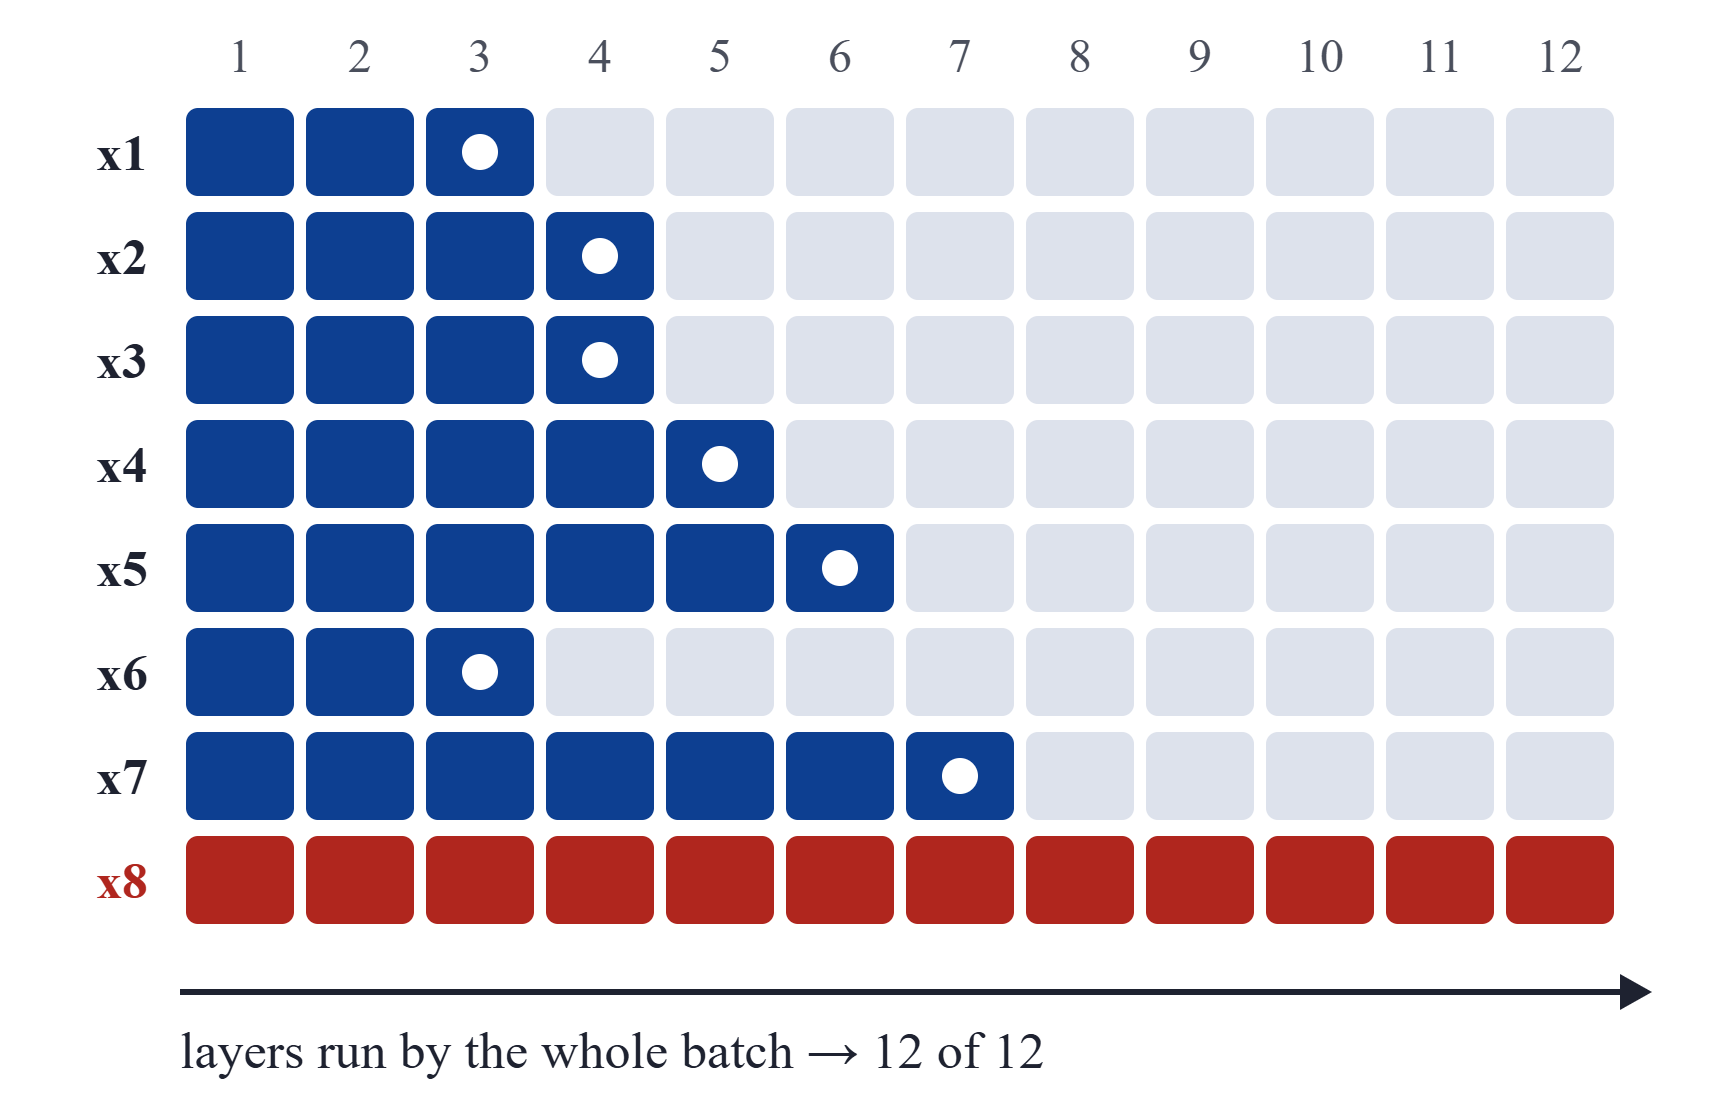
\includegraphics[width=\linewidth]{fig/straggler.png}
      {\scriptsize One batch of 8 inputs, 12 layers. Blue: computed; grey: idle (input already exited, $\circ$);
       red: the straggler.}
    \end{column}
    \begin{column}{0.51\textwidth}
      \small
      \begin{itemize}
        \item Early-exit networks let easy inputs stop at an intermediate layer \cite{deebert}.
        \item A GPU runs a batch layer by layer: one hard input keeps the whole batch running.
        \item Here the mean exit is layer 5.5, yet the batch pays for all 12.
        \item Existing batch rules (consensus, majority, greedy) are heuristics, not derived from the cost.
      \end{itemize}
    \end{column}
  \end{columns}
  \begin{block}{Questions}
    \small (1) When should a batch stop, and which exits are worth evaluating?
    (2) Can the rule be tuned with an accuracy guarantee?
    (3) Can slowdown attacks be bounded?
  \end{block}
\end{frame}

\begin{frame}{A stopping rule derived from the measured cost}
  \begin{block}{Cost model (measured on the GPU)}
    \vspace{-0.4em}
    \[ T(\text{batch}) \;=\; \sum_i \big[(d_i - d_{i-1})\,c(n_i) + h\big] \]
    {\footnotesize $d_i$: depth of the $i$-th exit evaluated, $n_i$: inputs still active, $h$: cost of one exit head.
     $c(n)$ has a floor ($\approx$1.8\,ms per RoBERTa layer on a GTX~1650); a straight line $a+bn$ errs by up to 41\%.}
  \end{block}
  \begin{block}{Rule: maximise accuracy $-\ \lambda\cdot$time}
    \small
    \begin{itemize}
      \item An input leaves alone if its expected gain from going deeper is below $\lambda\,[c(n)-c(n-1)]$.
      \item The remaining batch $R$ stops together if no later exit is worth $\lambda\,c(|R|)$.
      \item As the batch drains, the rule moves from per-input exits to whole-batch stopping.
    \end{itemize}
  \end{block}
  \footnotesize Tuning: record exit confidences $\to$ replay the rule on CPU for every $\lambda$ $\to$ \textbf{certify}: keep the
  fastest $\lambda$ that passes a $t$-test for an accuracy drop $\le 1$ point $\to$ deploy (a label-free bandit keeps
  tuning; a trimmed rule bounds attacks).
\end{frame}

\begin{frame}{Results: speed at matched accuracy}
  \begin{columns}[T]
    \begin{column}{0.46\textwidth}
      {\scriptsize\textbf{Speed-up over the full model, QQP, GTX 1650, timed}}\par
      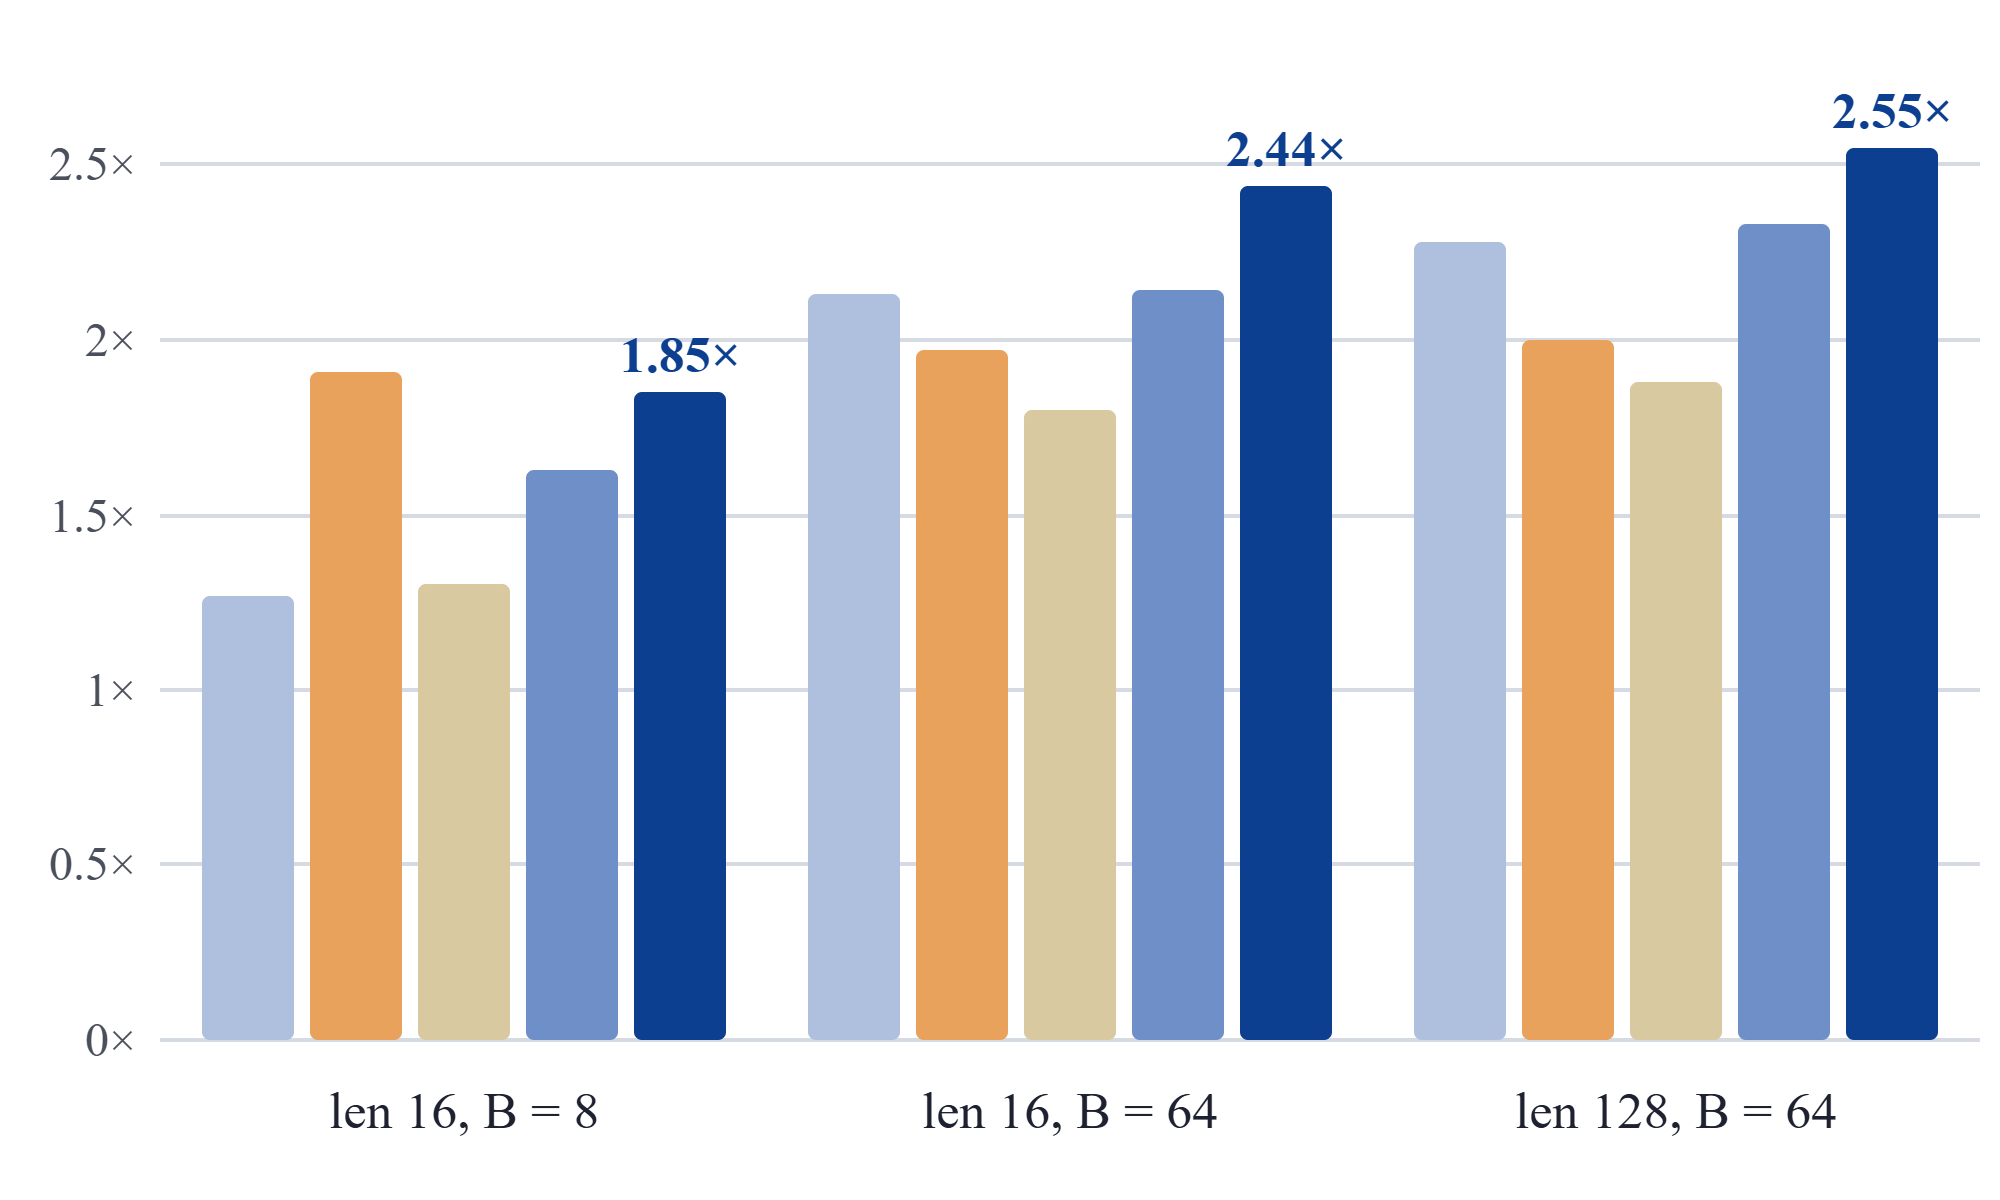
\includegraphics[width=\linewidth]{fig/speedup.png}\par
      {\tiny
       \textcolor[HTML]{AFC0DF}{$\blacksquare$}\,per-sample threshold\ \
       \textcolor[HTML]{E8A25E}{$\blacksquare$}\,unified exit\ \
       \textcolor[HTML]{D9CA9F}{$\blacksquare$}\,majority vote\\
       \textcolor[HTML]{7191C9}{$\blacksquare$}\,random search\ \
       \textcolor[HTML]{0F3F91}{$\blacksquare$}\,cost rule (ours)}
      \par\medskip
      {\scriptsize No fixed rule wins everywhere; ours is within 3\% of the fastest in 11 of 18 timed settings
       (best baseline: 5).}
    \end{column}
    \begin{column}{0.52\textwidth}
      {\scriptsize\textbf{At matched held-out accuracy (drop $\le$ 1 point), length 16}}\par\smallskip
      \scriptsize
      \begin{tabular}{@{}lccc@{}}
        \toprule
        & $B=8$ & $B=16$ & $B=64$ \\
        \midrule
        QQP, best baseline & 1.88$\times$ & 1.89$\times$ & 2.26$\times$ \\
        QQP, \ours{ours} & \ours{1.91$\times$} & \ours{2.13$\times$} & \ours{2.63$\times$} \\
        MNLI, best baseline & 1.49$\times$ & 1.49$\times$ & 1.66$\times$ \\
        MNLI, ours & 1.49$\times$ & 1.52$\times$ & 1.52$\times$ \\
        \bottomrule
      \end{tabular}
      \begin{itemize}\setlength\itemsep{2pt}
        \item QQP: ahead in all 6 settings by 2--17\%; RTX A6000 with trained weights: 8--14\% ahead.
        \item Llama-3.1-8B classifier on QQP: \ours{3.66$\times$} vs 3.50$\times$.
        \item RoBERTa on MNLI: within 2\% in 4 of 6 settings, 6.5--8.5\% behind in 2.
      \end{itemize}
    \end{column}
  \end{columns}
\end{frame}

\begin{frame}{Guarantees, attacks and limits}
  \begin{columns}[T]
    \begin{column}{0.49\textwidth}
      \begin{block}{What holds}
        \footnotesize
        \begin{itemize}
          \item Certified selection: 0--7\% of random re-splits exceed the 1-point budget (plain tuning: 13--40\%).
          \item Slowdown bound never broken: 0 of 25{,}200 attacked batches; majority and consensus fall to $\approx 1\times$.
          \item The collective stop is provably optimal in the monotone case; exact dynamic programming agrees in
                210 of 210 instances.
          \item The label-free bandit has sublinear regret ($t^{0.55}$--$t^{0.77}$, 10 seeds).
        \end{itemize}
      \end{block}
    \end{column}
    \begin{column}{0.49\textwidth}
      \begin{alertblock}{What does not}
        \footnotesize
        \begin{itemize}
          \item The accuracy loss lands on hard inputs: 2.0--2.7 points on the hardest quarter of MNLI.
          \item LLM decoders: the gain shrinks from 12\% at batch 1 to 0.2\% at batch 64.
          \item The finite-sample certificate is too loose to certify anything.
        \end{itemize}
      \end{alertblock}
    \end{column}
  \end{columns}
  \vfill
  \small Lesson we carried forward: search (by an LLM or otherwise) pays off where answers can be
  \emph{checked exactly}. That led us to index coding.
\end{frame}

% ================================================================= 2
\section{From early exit to minrank: Kneser graphs}

\begin{frame}{Index coding, minrank and Kneser graphs}\label{fr:kneser}
  \begin{columns}[T]
    \begin{column}{0.58\textwidth}
      \begin{block}{Index coding \cite{baryossef}}
        \footnotesize A sender holds one message per receiver. Receiver $v$ wants its own message and already knows the
        messages of its neighbours in a graph $G$. How few broadcasts suffice?
      \end{block}
      \vspace{-0.3em}
      {\footnotesize\[ \underbrace{\alpha(G)}_{\text{lower bound}} \le \underbrace{\beta(G)}_{\text{optimum}}
         \le \underbrace{\operatorname{minrk}_{F}(G)}_{\text{best linear code}}
         \le \underbrace{\bar\chi(G)}_{\text{clique cover}} \]}
      \begin{block}{Kneser graph $K(n,k)$}
        \footnotesize Receivers: all $k$-element subsets of $\{1,\dots,n\}$; two are adjacent iff disjoint.
        Here $\alpha=\binom{n-1}{k-1}$ (Erd\H{o}s--Ko--Rado): the sets containing 1.
      \end{block}
    \end{column}
    \begin{column}{0.40\textwidth}
      \centering
      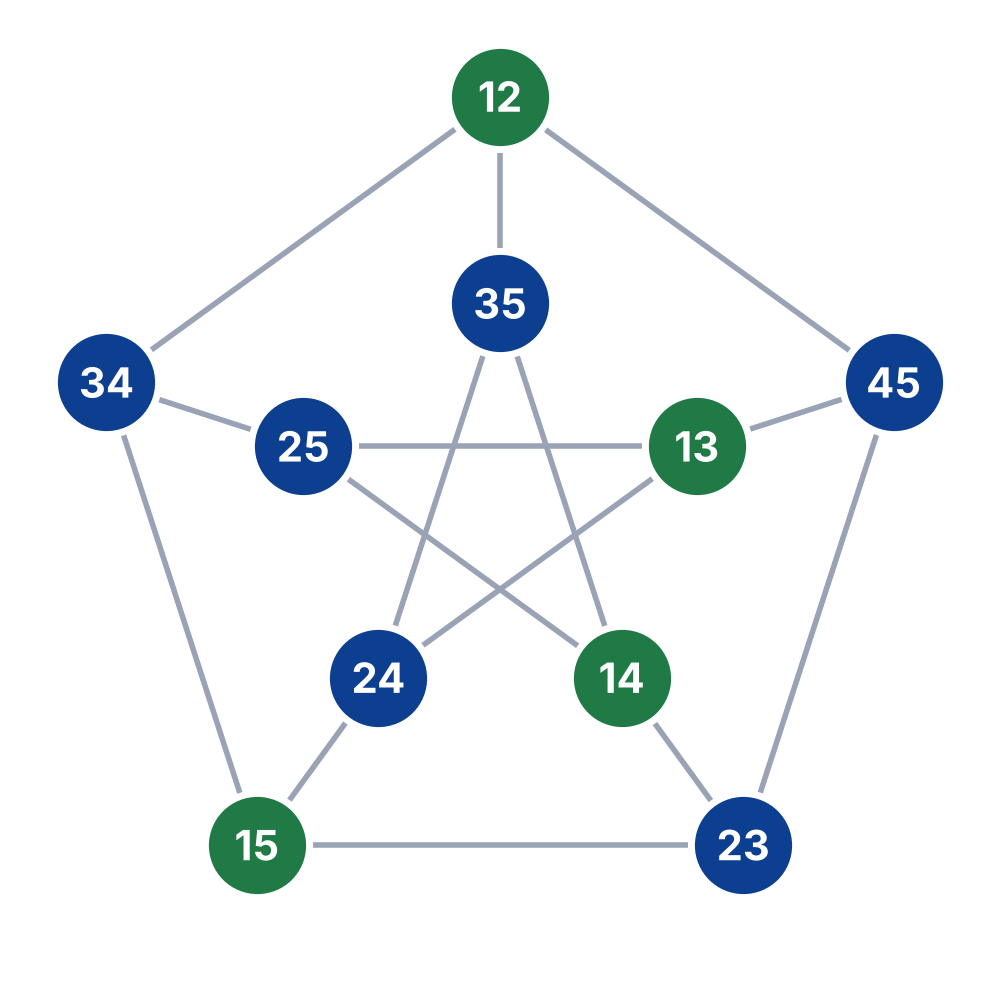
\includegraphics[width=0.95\linewidth]{fig/k52.png}\par
      {\scriptsize $K(5,2)$: 10 receivers. Green: the 4 pairs containing 1, no two adjacent, so $\alpha = 4$.}
    \end{column}
  \end{columns}
  \vfill
  {\small Exact $\beta$ is known for very few graph families.}
\end{frame}

\begin{frame}{Our result: exact minrank of Kneser graphs}
  \begin{theorem}[ours]
    Let $p$ be a prime and $q$ the least power of $p$ with $q \ge k$. With $D$ the disjointness matrix of $K(n,k)$,
    \[ \operatorname{rank}_{\Fp}(I \pm D) = \binom{n-1}{k-1} \iff q \mid n-2k . \]
    Hence $\operatorname{minrk}_{\Fp}(K(n,k)) = \beta = \alpha$ in these cases, with an explicit optimal code: for each
    set $A \ni 1$, broadcast $x_A \pm \sum_{B \cap A = \emptyset} x_B$.
  \end{theorem}
  \begin{itemize}\small
    \item $\beta(K(n,k)) = \alpha$ for all but finitely many $n$, for every $k$.
    \item The field matters: $\operatorname{minrk}(K(7,2)) = 7$ over $\mathbb{F}_2$ but $6$ over $\mathbb{F}_3$
          (SAT, DRAT-checked).
    \item New for $k \nmid n$ (for $k \mid n$ it follows from Baranyai's theorem); there even the fractional clique
          cover exceeds $\alpha$.
    \item Elementary proof (star basis and Lucas' theorem); checked by exact rank in 318 cases.
  \end{itemize}
\end{frame}

% ================================================================= 3
\section{An agent that proves $\beta$}

\begin{frame}{Why an agent?}
  \begin{columns}[T]
    \begin{column}{0.49\textwidth}
      \begin{alertblock}{Proving $\beta$ gets slow}
        \footnotesize
        \begin{itemize}
          \item Standard methods (CP-SAT, clique cover, $\mathbb{F}_2$ SAT): \textbf{2 of 25} benchmark graphs proven in
                60\,s each.
          \item One certified rank check costs $\approx N^2 r$: on $N = 14{,}950$ receivers, 54\,s.
          \item Real inputs arrive unlabelled: vertices shuffled, no family name.
        \end{itemize}
      \end{alertblock}
    \end{column}
    \begin{column}{0.49\textwidth}
      \begin{block}{Idea}
        \footnotesize
        \begin{itemize}
          \item An LLM reads a numeric summary of the graph, guesses its structure and plans which certified checks
                to run.
          \item Worker processes run the checks in parallel; the run stops the moment lower bound $=$ upper bound.
          \item Only certified results count; an independent verifier re-checks the final code.
        \end{itemize}
      \end{block}
    \end{column}
  \end{columns}
  \vfill
  \begin{block}{Baseline: the Kneser agent (no LLM)}
    \footnotesize A fixed script: recognise $(n,k)$ from vertex count and degree $\to$ the theorem names the prime
    $\to$ one exact rank (FLINT library) $\to$ greedy independent set $\to$ otherwise fall back to a general solver.
  \end{block}
\end{frame}

\begin{frame}{Kneser agent (no LLM) vs our LLM agent}
  \scriptsize
  \renewcommand{\arraystretch}{1.25}
  \begin{tabularx}{\textwidth}{@{}>{\raggedright\arraybackslash}p{1.75cm}LL@{}}
    \toprule
    & \textbf{Kneser agent (no LLM)} & \textbf{Our LLM agent} \\
    \midrule
    Input & adjacency matrix & same matrix, vertices shuffled; the LLM sees only a numeric summary \\
    Decision & 5 fixed steps & Solver LLM: hypothesis $+$ plan; Critic LLM challenges it (up to 3 rounds) \\
    Field choice & from the theorem only & theorem as one tool, plus a generic rule from the eigenvalues and any $(p,c)$ \\
    Execution & one step after another & scheduler with 3 worker processes; retargets on new bounds, stops when they meet \\
    Wrong guess & fall back to the general solver & checkpoint: the Solver sees the results and revises the plan \\
    Rank check & full exact rank, $O(N^3)$ & rank factorisation with early stop, $O(N^2 r)$ \\
    Checking & certificates re-checked in the same code & independent verifier code (shares nothing with the tools) \\
    Fixed cost & none (0.02\,s on small graphs) & LLM thinking, $\approx$20--40\,s per graph \\
    \bottomrule
  \end{tabularx}
\end{frame}

\begin{frame}{Agentic workflow}
  \centering
  \begin{tikzpicture}[
      x=1cm, y=1cm, font=\scriptsize, >={Stealth[length=2mm]},
      box/.style={rounded corners=2pt, minimum width=2.5cm, minimum height=1.45cm, align=center, text width=2.35cm,
                  inner sep=2pt},
      llm/.style={box, fill=structure.fg, text=white},
      code/.style={box, fill=structure.fg!7, draw=structure.fg!70},
      res/.style={box, fill=green!40!black, text=white},
      lab/.style={font=\tiny, align=center, text=black!75}]
    \node[code] (g)  at (0,0)     {\textbf{Graph}\\shuffled, no name};
    \node[code] (s)  at (2.85,0)  {\textbf{Summary tools}\\receivers, degrees, eigenvalues, greedy bounds};
    \node[llm]  (so) at (5.7,0)   {\textbf{Solver (LLM)}\\family hypothesis $+$ plan of tool calls};
    \node[llm]  (cr) at (8.55,0)  {\textbf{Critic (LLM)}\\checks every number; accept or challenge};
    \node[code] (w)  at (2.85,-2.3) {\textbf{3 workers}\\codes $I+cA$ over $\Fp$, independent sets, covers};
    \node[code] (sc) at (5.7,-2.3)  {\textbf{Scheduler}\\new bound $\to$ retarget; near miss $\to$ more $c$};
    \node[code] (bd) at (8.55,-2.3) {\textbf{Bound board}\\certified lower $\le \beta \le$ upper};
    \node[llm]  (ve) at (8.55,-4.6) {\textbf{Verifier}\\own code re-checks; LLM writes report};
    \node[res]  (o)  at (5.7,-4.6)  {\textbf{$\beta$ $+$ optimal code}\\verdict from the checks};
    \draw[->] (g) -- (s);
    \draw[->] (s) -- (so);
    \draw[->] ([yshift=2mm]so.east) -- ([yshift=2mm]cr.west);
    \draw[->] ([yshift=-2mm]cr.west) -- ([yshift=-2mm]so.east);
    \node[lab] at (7.125,0.95) {up to 3 rounds};
    \draw[->] ([xshift=-4mm]so.south) -- node[lab, left] {accepted plan} ([xshift=-4mm]sc.north);
    \draw[->] ([yshift=2mm]sc.west) -- ([yshift=2mm]w.east);
    \draw[->] ([yshift=-2mm]w.east) -- ([yshift=-2mm]sc.west);
    \draw[->] (sc) -- node[lab, above] {results} (bd);
    \draw[->, dashed] ([xshift=-8mm]bd.north) -- node[lab, right, pos=0.5, xshift=1mm] {plan exhausted: checkpoint} ([xshift=8mm]so.south);
    \draw[->] (bd) -- node[lab, right] {bounds meet} (ve);
    \draw[->] (ve) -- (o);
    \node[anchor=north west, text width=4.6cm, font=\scriptsize] at (-1.25,-3.95)
      {\tikz\fill[structure.fg] (0,0) rectangle (0.25,0.18);\ LLM agent\quad
       \tikz{\fill[structure.fg!7] (0,0) rectangle (0.25,0.18); \draw[structure.fg!70] (0,0) rectangle (0.25,0.18);}\ code\\[3pt]
       The LLMs never write a number to the board: only certified tool results enter.};
  \end{tikzpicture}
\end{frame}

\begin{frame}{Results: time to prove $\beta$ (container, one CPU core per run)}
  \centering
  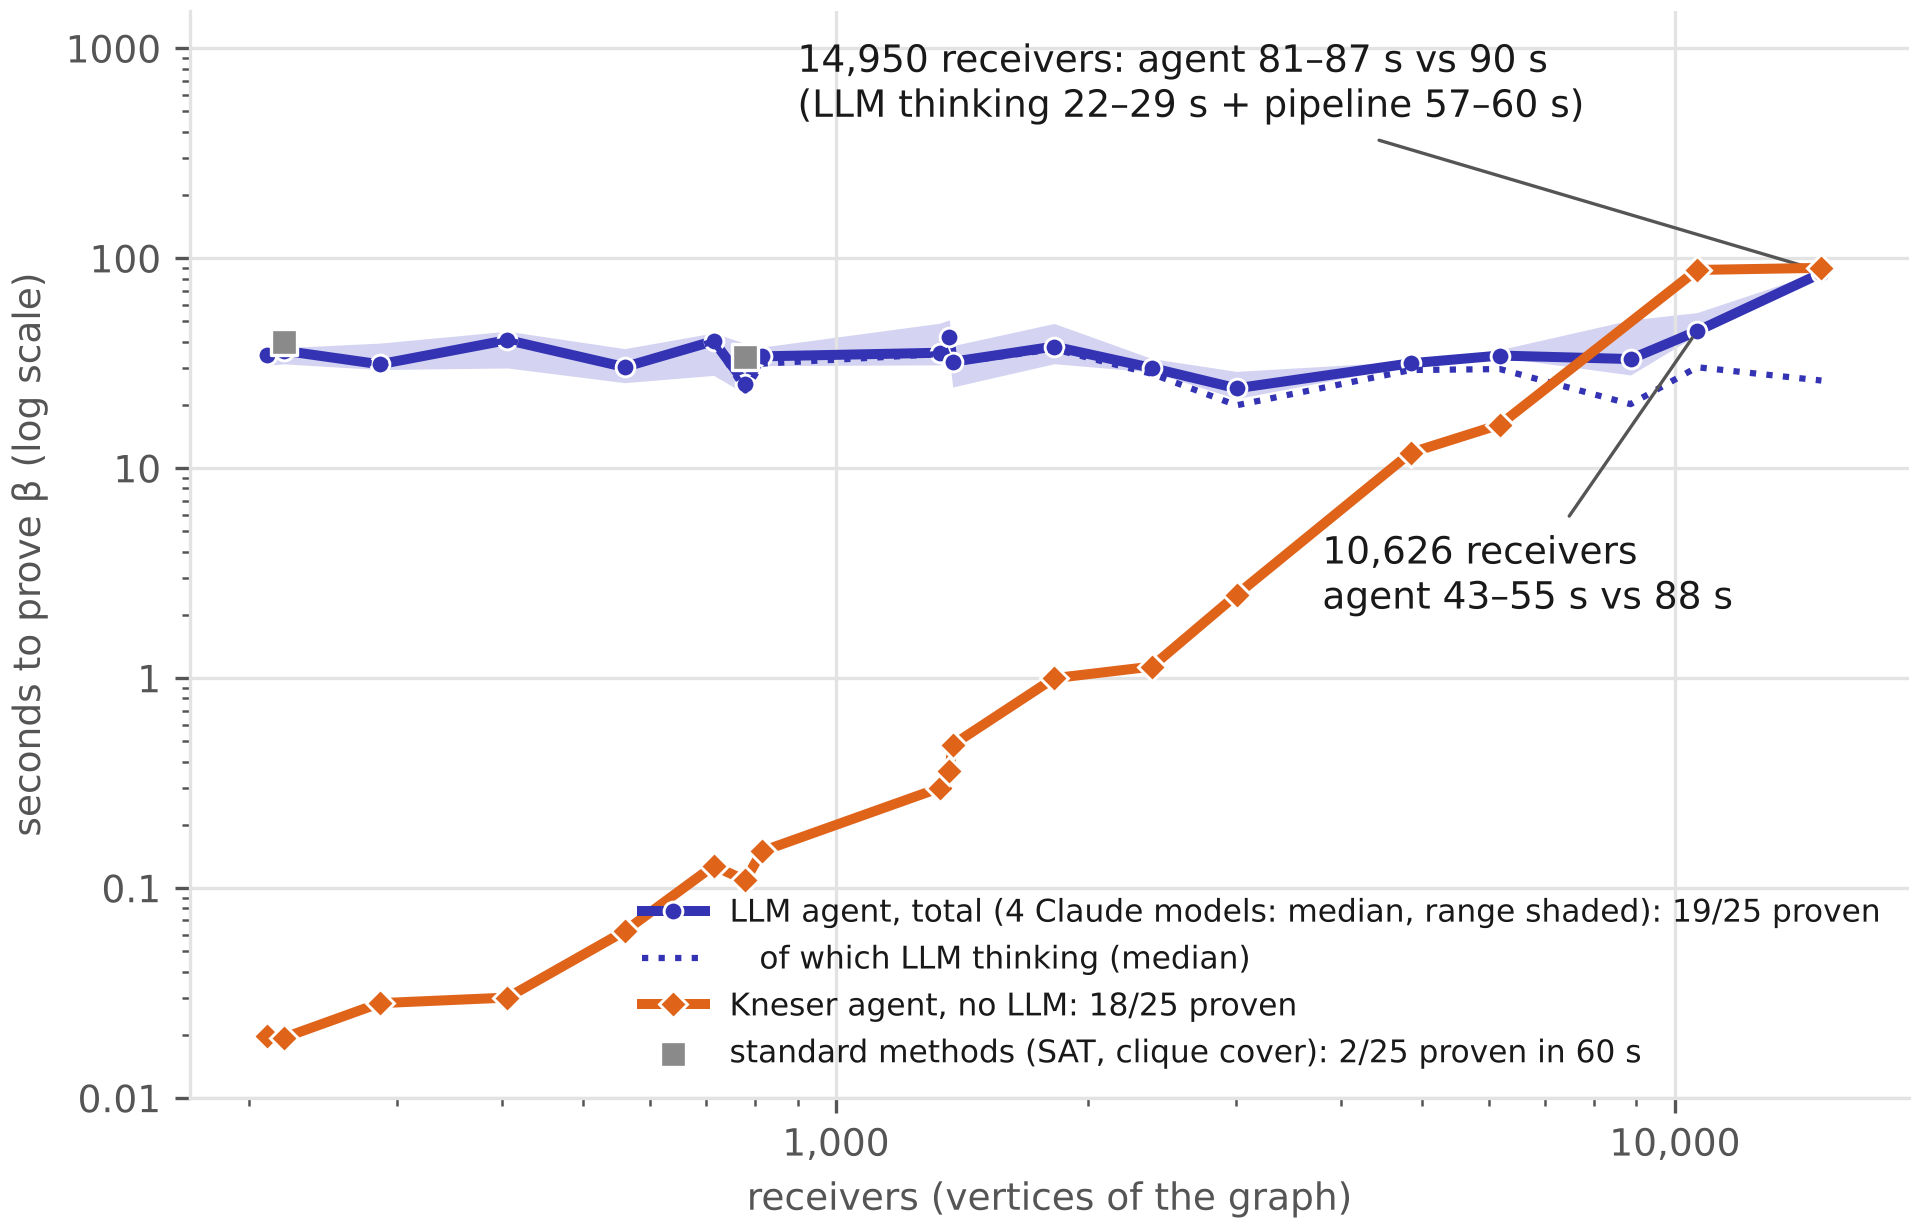
\includegraphics[width=0.80\linewidth]{fig/time_to_prove_beamer.png}\par
  \vspace{-0.2em}
  {\tiny Time until the certified bounds meet, LLM time included; 20 benchmark graphs $+$ 5 large Kneser graphs, seed 0.
   Claude LLM time is the wall time of a Claude Code agent (tool calls included), so it overstates pure model time.\par}
  \vspace{0.2em}
  \begin{alertblock}{Takeaway}
    \scriptsize LLM thinking stays at $\approx$20--40\,s while compute grows. Below $\approx$9{,}000 receivers the script
    is faster; at 10{,}626 receivers the agent needs 43--55\,s vs 88\,s, at 14{,}950 it needs 81--87\,s vs 90\,s.
  \end{alertblock}
\end{frame}

\begin{frame}{Model ablation: which LLM drives the agent}
  \small
  One fresh, blind agent per graph (it never sees the graph's name); same prompts for every model.\par\medskip
  \centering
  \footnotesize
  \begin{tabular}{@{}lcccc@{}}
    \toprule
    & & & \multicolumn{2}{c}{time at $N$ receivers} \\ \cmidrule(l){4-5}
    LLM (effort) & proven & median & 10{,}626 & 14{,}950 \\
    \midrule
    Claude Sonnet 5.5 (medium) & 19/25 & 31.5\,s & 45.5\,s & 83.5\,s \\
    Claude Opus 5.5 (low)      & 19/25 & 31.0\,s & 44.4\,s & 86.7\,s \\
    Claude Opus 5.5 (medium)   & 19/25 & 35.9\,s & 43.1\,s & 81.1\,s \\
    Claude Opus 5.5 (high)     & 19/25 & 38.3\,s & 55.0\,s & 86.2\,s \\
    \midrule
    Qwen2.5-Coder-32B (GPU) & 17/23 & 40.9\,s & -- & -- \\
    Kneser agent (no LLM)      & 18/25 & 0.3\,s & 87.9\,s & 89.9\,s \\
    \bottomrule
  \end{tabular}
  \raggedright
  \begin{itemize}\footnotesize
    \item All four Claude settings prove the same 19 graphs; more effort only adds time.
    \item The 6 graphs left open (exceptions of the theorem, perturbed and random graphs) stay open for every method.
  \end{itemize}
\end{frame}

% ================================================================= 4
\section{Conclusions}

\begin{frame}{Conclusions}
  \begin{block}{Early exit}
    \footnotesize The fastest rule changes with batch size and input length; a rule derived from the measured cost tracks
    it. At matched accuracy it leads on QQP (2--17\%) and on Llama classifiers (3.66$\times$); certified selection keeps the
    1-point budget and the slowdown bound never broke. No gain on RoBERTa MNLI or on LLM decoders.
  \end{block}
  \begin{block}{Minrank}
    \footnotesize $\operatorname{minrk}_{\Fp}(K(n,k)) = \beta = \alpha$ exactly when $q \mid n-2k$, with an explicit optimal
    index code; new for $k \nmid n$. Small cases such as $K(9,2)$ over $\mathbb{F}_2$ remain open.
  \end{block}
  \begin{block}{Agent}
    \footnotesize A Solver--Critic--Verifier pipeline proves $\beta$ blind on 19 of 25 graphs with every Claude model, and
    beats the Kneser script at 10{,}626 receivers (43--55\,s vs 88\,s). Its LLM costs a near-constant 20--40\,s, so it
    pays off only on large graphs.
  \end{block}
\end{frame}

\begin{frame}{References}
  \scriptsize
  \begin{thebibliography}{10}
    \bibitem{deebert} J.~Xin et al., ``DeeBERT: Dynamic early exiting for accelerating BERT inference,'' ACL, 2020.
    \bibitem{drex} X.~Liu et al., ``Dynamic rebatching for efficient early-exit inference with DREX,'' arXiv:2512.15705, 2025.
    \bibitem{apparate} Y.~Dai et al., ``Apparate: Rethinking early exits to tame latency-throughput tensions in ML serving,'' SOSP, 2024.
    \bibitem{ltt} A.~N.~Angelopoulos et al., ``Learn then Test: Calibrating predictive algorithms to achieve risk control,'' arXiv:2110.01052, 2021.
    \bibitem{chow} Y.~S.~Chow, H.~Robbins, D.~Siegmund, \emph{Great Expectations: The Theory of Optimal Stopping}, 1971.
    \bibitem{ceebert} D.~J.~Bajpai, M.~K.~Hanawal, ``CeeBERT: Cross-domain inference in early exit BERT,'' Findings of ACL, 2024.
    \bibitem{sloth} S.~Hong et al., ``A Panda? No, it's a Sloth: Slowdown attacks on adaptive multi-exit neural network inference,'' ICLR, 2021.
    \bibitem{baryossef} Z.~Bar-Yossef, Y.~Birk, T.~S.~Jayram, T.~Kol, ``Index coding with side information,'' IEEE Trans.\ Inf.\ Theory, 2011.
    \bibitem{gh} A.~Golovnev, I.~Haviv, ``The (generalized) orthogonality dimension of (generalized) Kneser graphs,'' Theory of Computing, 2022.
    \bibitem{ducey} J.~Ducey et al., ``Integer diagonal forms for subset intersection relations,'' 2024.
  \end{thebibliography}
\end{frame}

\begin{frame}
  \centering
  \vfill
  {\Huge\color{structure.fg} Thank you}\par\bigskip
  {\large Questions?}\par\vfill
  {\footnotesize Appendix: agent system prompts, model ablation, proof sketch, worked example, evidence.}
\end{frame}

% ================================================================= appendix
\appendix

\begin{frame}[fragile]{Appendix A1: Solver system prompt (verbatim)}
  \lstinputlisting{prompts/solver.txt}
\end{frame}

\begin{frame}[fragile]{Appendix A2: Critic and checkpoint prompts (verbatim)}
  \lstinputlisting{prompts/critic.txt}
\end{frame}

\begin{frame}[fragile]{Appendix A3: Verifier system prompt (verbatim)}
  \lstinputlisting{prompts/verifier.txt}
  \footnotesize Every reply is validated by code: JSON schema, known tool names, integer arguments, a prime $p$; every
  evidence item must quote a number the agent was given, and every ``$C(a,b) = X$'' is recomputed. An invalid reply is
  returned once with the error; a second failure falls back to a deterministic default plan.
\end{frame}

\begin{frame}[fragile]{Appendix A4: Tool list appended to the Solver and Critic prompts}
  \lstinputlisting{prompts/tools.txt}
  \footnotesize Prompt version v4. The LLM chooses and orders tools, argues and explains; it never writes a bound.
\end{frame}

\begin{frame}{Appendix A5: Time to prove $\beta$ for each LLM}
  \centering
  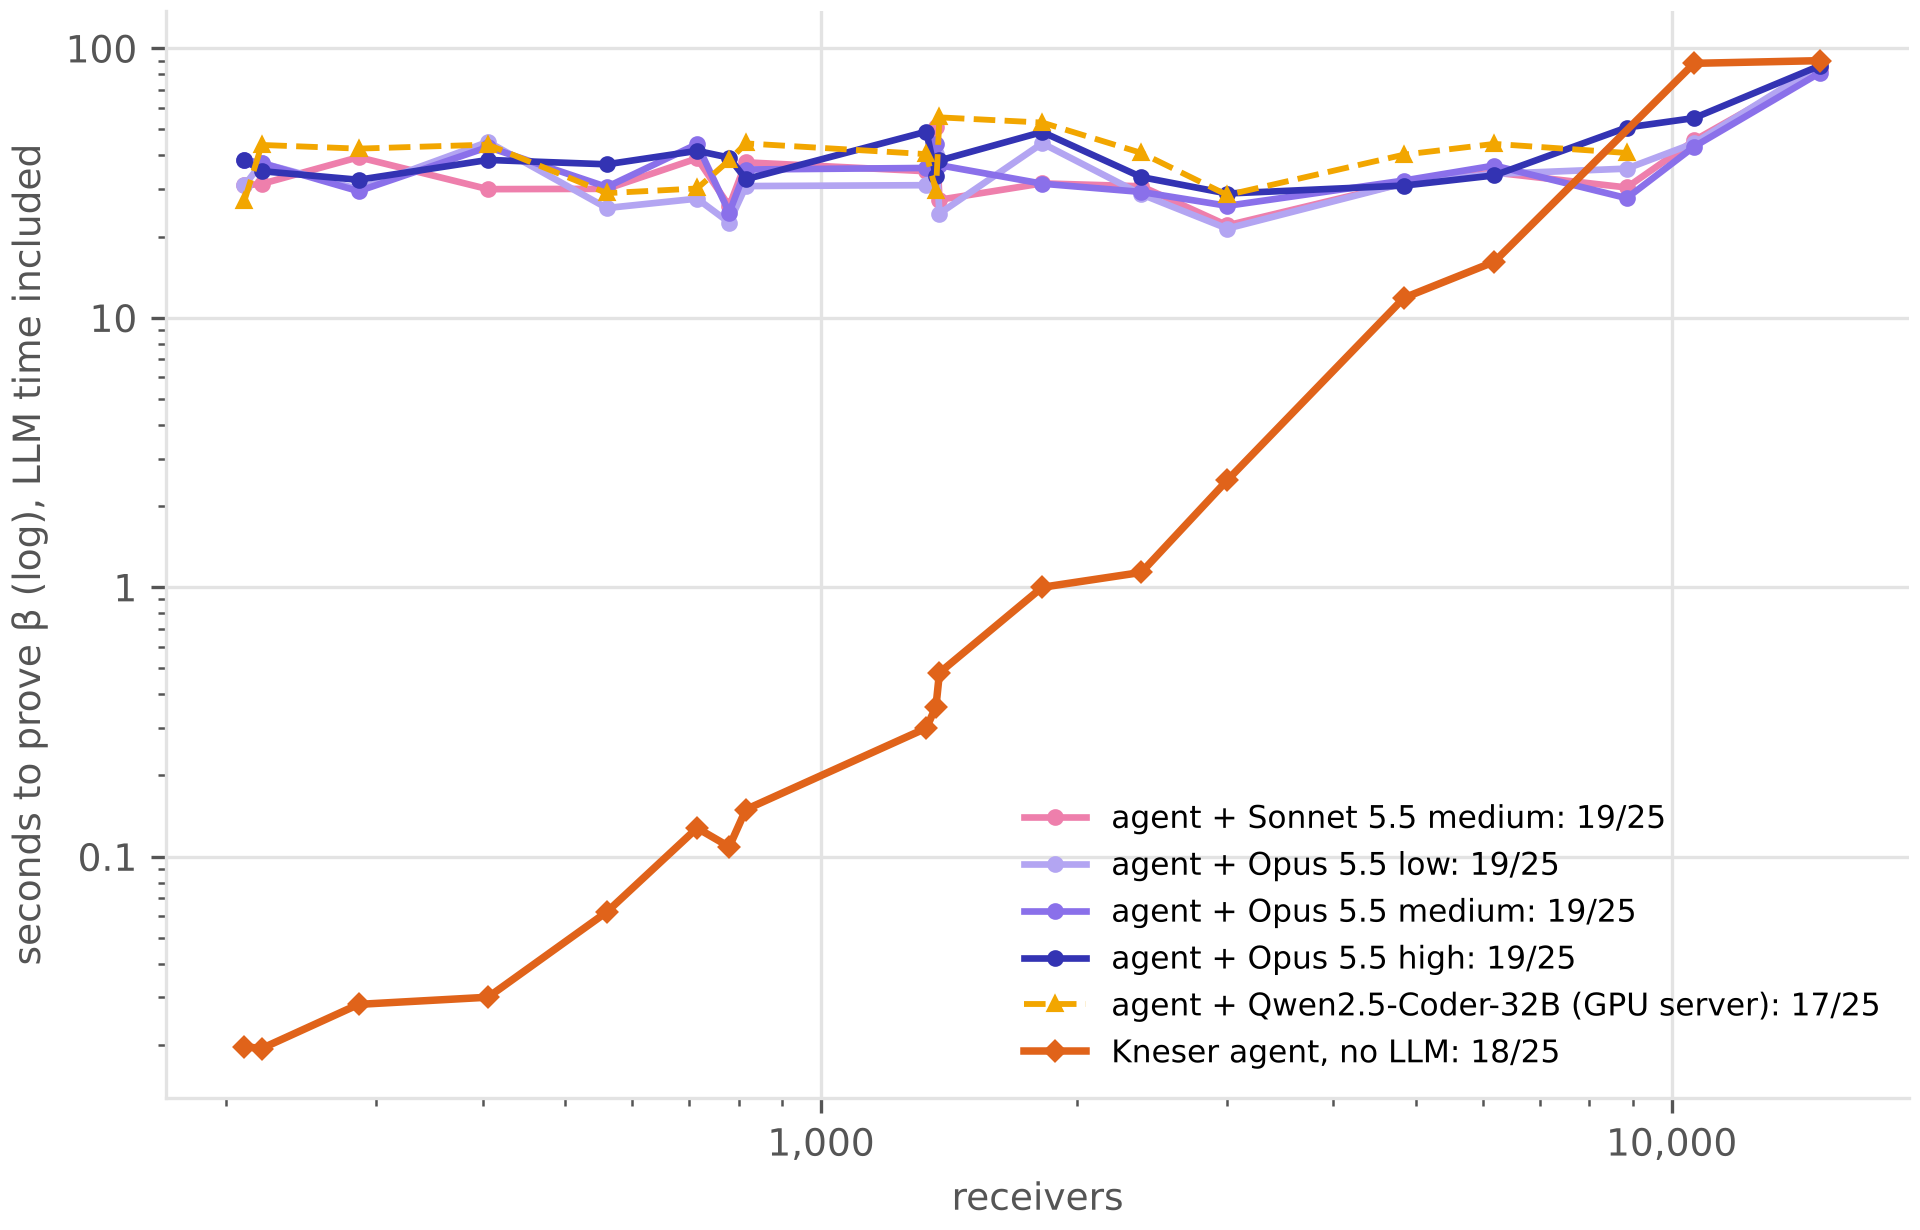
\includegraphics[width=0.92\linewidth]{fig/time_to_prove_models_beamer.png}
\end{frame}

\begin{frame}{Appendix A6: Proof sketch of the theorem}
  \footnotesize $H = I + \varepsilon D$ with $\varepsilon = (-1)^{k-1}$; $N = n-2k$; $S = \{A : 1 \in A\}$ (the star).
  \begin{enumerate}
    \item \textbf{Star rows are independent.} $H$ restricted to $S$ is the identity, so $\operatorname{rank} H \ge \alpha$
          over every field.
    \item \textbf{Decoding identity.} For $A' \notin S$, compare row $A'$ with $\varepsilon\sum_{A \in S,\,A\cap A'=\emptyset}$
          row $A$: they agree on columns $B \ni 1$; on $B \not\ni 1$ they differ by $\binom{N-1+t}{k-1}$ vs
          $\binom{t-1}{k-1}$, $t = |A' \cap B|$.
    \item \textbf{Rank $\alpha$ iff a congruence.} $\operatorname{rank}_p H = \alpha$ iff
          $\binom{N-1+t}{k-1} \equiv \binom{t-1}{k-1} \pmod p$ for $t = 0,\dots,k$.
    \item \textbf{Lucas' theorem.} Vandermonde turns this into $\binom{N}{i} \equiv 0 \pmod p$ for $1 \le i \le k-1$,
          which holds iff $q_p(k) \mid N$.
  \end{enumerate}
  Since $H$ fits $K(n,k)$ (zero on non-adjacent pairs, nonzero diagonal), $\operatorname{minrk}_{\Fp} = \alpha$ exactly in
  those cases; $\alpha$ is a lower bound for every index code, so the linear code is optimal.
\end{frame}

\begin{frame}{Appendix A7: Worked example, an optimal code for $K(7,2)$ over $\mathbb{F}_3$}
  \footnotesize
  \begin{columns}[T]
    \begin{column}{0.44\textwidth}
      \begin{tabular}{@{}lr@{}}
        \toprule
        Receivers (pairs from $1..7$) & 21 \\
        $q_3(2) = 3$ divides $7-4$? & yes \\
        Our code: broadcasts $= \alpha$ & 6 \\
        Clique-cover code & 7 \\
        Best linear code over $\mathbb{F}_2$ & 7 \\
        \bottomrule
      \end{tabular}
    \end{column}
    \begin{column}{0.54\textwidth}
      \textbf{Encoder} ($\varepsilon = -1$): for each pair $A = \{1,j\}$ broadcast
      $y_A = x_A - \sum_{B \cap A = \emptyset} x_B \pmod 3$.\par\smallskip
      \textbf{Receiver $\{1,4\}$} knows every $x_B$ with $B$ disjoint from it, so it reads $x_{14}$ from $y_{14}$.\par\smallskip
      \textbf{Receiver $\{2,3\}$} computes $-(y_{14}+y_{15}+y_{16}+y_{17}) = x_{23} - \sum_{B\cap\{2,3\}=\emptyset} x_B$
      and removes the sum it knows.
    \end{column}
  \end{columns}
  \medskip
  Checked numerically on random messages. Over $\mathbb{F}_2$ no 6-broadcast linear code exists (SAT, DRAT-checked).
\end{frame}

\begin{frame}{Appendix A8: Which cases are new}
  \footnotesize
  \begin{columns}[T]
    \begin{column}{0.52\textwidth}
      \textbf{New: $k \nmid n$, no clique cover reaches $\alpha$}\par\smallskip
      \begin{tabular}{@{}llrr@{}}
        \toprule
        Graph & Field & $\operatorname{minrk} = \alpha$ & frac.\ cover \\
        \midrule
        $K(7,2)$ & $\mathbb{F}_3$ & 6 & 7 \\
        $K(10,3)$ & $\mathbb{F}_2$ & 36 & 40 \\
        $K(13,4)$ & $\mathbb{F}_5$ & 220 & 238.3 \\
        $K(15,4)$ & $\mathbb{F}_7$ & 364 & 455 \\
        \bottomrule
      \end{tabular}\par\medskip
      Infinitely many for every $k$: take a prime $p > k$ and $n = 2k + pt$ with $t \equiv 1 \pmod k$.
    \end{column}
    \begin{column}{0.44\textwidth}
      \textbf{$n$ not covered by any prime}\par\smallskip
      \begin{tabular}{@{}cl@{}}
        \toprule
        $k$ & $n$ \\
        \midrule
        2 & 5 \\
        3 & 7, 8 \\
        4 & 9, 10, 11, 14 \\
        5 & 11, 12, 13, 14, 16, 22 \\
        \bottomrule
      \end{tabular}\par\medskip
      Known before: for $k \mid n$, Baranyai's theorem gives $\alpha$ perfect matchings, so $\operatorname{minrk} = \alpha$
      over every field.
    \end{column}
  \end{columns}
\end{frame}

\begin{frame}{Appendix A9: Evidence and computer proofs}
  \footnotesize
  \begin{itemize}
    \item 318 $(n,k,p)$ cases: rank $= \alpha$ exactly when $q \mid n-2k$; 82 of them checked by two independent rank codes
          (39 with $k \nmid n$).
    \item 6{,}666 cases of a second proof via integer diagonal forms \cite{ducey} agree.
    \item $\operatorname{minrk}(K(7,2))$: 7 over $\mathbb{F}_2$ vs 6 over $\mathbb{F}_3$; the $\mathbb{F}_2$ lower bound is a
          DRAT-checked SAT proof.
    \item $\operatorname{minrk}_{\mathbb{F}_2}$ of $K(7,3)$ and $K(8,3)$ is 18 and 22, above $\alpha = 15, 21$ (DRAT-checked).
    \item Open: $K(9,2)$, $K(11,2)$ over $\mathbb{F}_2$; a star-basis SAT reduction (0.3\,s on $K(7,2)$, was over 1\,h)
          did not finish in 2\,h.
    \item Agent runs: every proven code is re-checked by the verifier's own code (fit, exact factorisation
          $M = M[:,S]\,M[S,:]$, own elimination, decoding simulation).
  \end{itemize}
\end{frame}

\begin{frame}{Appendix A10: Likely questions}
  \fontsize{6.6}{7.6}\selectfont
  \begin{description}[Why is a linear code optimal?]
    \item[Is the theorem known?] Exact values were known only for $k \mid n$ (Baranyai); Golovnev--Haviv \cite{gh} and Haviv
          give bounds.
    \item[If $q \nmid n-2k$?] Then this $H$ has rank above $\alpha$; we do not claim $\operatorname{minrk} > \alpha$.
    \item[Why is a linear code optimal?] Any index code needs at least $\alpha$ broadcasts; ours uses exactly $\alpha$.
    \item[Does the agent need the theorem?] No: it is one tool the Solver may query; a generic eigenvalue rule and
          arbitrary $(p,c)$ codes are also available, and every result is certified.
    \item[Is the LLM time fair?] It is wall time of a Claude Code agent answering one request file, tool calls included,
          so it overstates model latency; the pipeline's later independent re-verification is not counted for either method.
    \item[Why is the agent faster at 10{,}626?] Its rank engine stops once the rank is certified ($O(N^2 r)$), while the
          script computes a full exact rank ($O(N^3)$). The LLM chooses the right field and constant, and the rank engine
          makes the check cheap.
    \item[How did we get to minrank?] In early exit, LLM program search only tied our rule; the Pincer agent on minrank
          closed 13 of 26 unseen graphs vs 2 for the classic pipeline, and its data showed the Kneser pattern.
  \end{description}
\end{frame}

\end{document}
